\documentclass[a4paper,12pt]{article}

\usepackage{tikz}
\usetikzlibrary{shapes.geometric,shapes.misc}
\usetikzlibrary{arrows}
\usepackage{mathrsfs}


\tikzset{
  term/.style={
    % The shape:
    shape=rectangle,rounded corners=3mm,
    % The size:
    minimum size=6mm,
    % The border:
    very thick,
    draw=red!50!black!50, % 50% red and 50% black,
    % and that mixed with 50% white
    % The filling:
    top color=white, % a shading that is white at the top...
    bottom color=red!50!black!20 % and something else at the bottom
  }}

\tikzset{
	nterm/.style={
		% The shape:
		rectangle,minimum size=6mm,rounded corners=3mm,
		% The rest
		very thick,draw=black!30,
		top color=black!05,bottom color=black!10,
		font=\ttfamily}}



\begin{document}


% Binomial tree
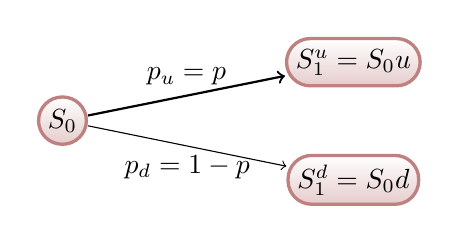
\begin{tikzpicture}
	\matrix (tree) [column sep=25mm, row sep=1mm]{
		& \node[term] (u) {$S_1^u = S_0u$}; \\
		\node[term] (s) {$S_0$}; \\
		& \node[term] (d) {$S_1^d = S_0d$}; \\
	};
	\draw[->,thick] (s) -- (u) node[midway,above] {$p_u = p$};
	\draw[->] (s) -- (d) node[midway,below] {$p_d = 1-p$};
\end{tikzpicture}


% Recombining 4-step binomial tree for Cox-Ross-Rubinstein model
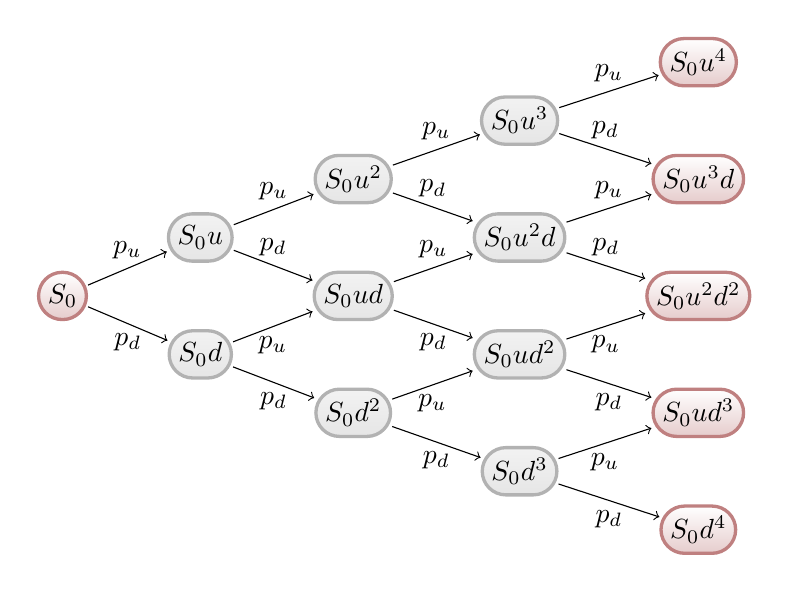
\begin{tikzpicture}
	\matrix[column sep=10mm,row sep=1mm] (tree){
		& & & & \node[term] (u4) {$S_0u^4$}; \\
		& & & \node[nterm] (u3) {$S_0u^3$}; & \\
		& & \node[nterm] (u2) {$S_0u^2$}; & & \node[term] (u3d) {$S_0u^3d$}; \\
		& \node[nterm] (u) {$S_0u$}; & & \node[nterm] (u2d) {$S_0u^2d$};\\
		\node[term] (s) {$S_0$}; & & \node[nterm] (ud) {$S_0ud$}; & & \node[term] (u2d2) {$S_0u^2d^2$}; \\
		& \node[nterm] (d) {$S_0d$}; & &	\node[nterm] (ud2) {$S_0ud^2$};\\
		& & \node[nterm] (d2) {$S_0d^2$}; & & \node[term] (ud3) {$S_0ud^3$}; \\
		& & & \node[nterm] (d3) {$S_0d^3$}; & \\
		& & & & \node[term] (d4) {$S_0d^4$}; \\
	};
	% Lines out of s
	\draw[->] (s) -- (u) node[midway,above] {$p_u$};
	\draw[->] (s) -- (d) node[midway,below] {$p_d$};
	% Lines out of u
	\draw[->] (u) -- (u2) node[midway,above] {$p_u$};
	\draw[->] (u) -- (ud) node[midway,above] {$p_d$};
	% Lines out of d
	\draw[->] (d) -- (ud) node[midway,below] {$p_u$};
	\draw[->] (d) -- (d2) node[midway,below] {$p_d$};
	% Lines out of u2
	\draw[->] (u2) -- (u3) node[midway,above] {$p_u$};
	\draw[->] (u2) -- (u2d) node[midway,above] {$p_d$};
	% Lines out of ud
	\draw[->] (ud) -- (u2d) node[midway,above] {$p_u$};
	\draw[->] (ud) -- (ud2) node[midway,below] {$p_d$};
	% Lines out of d2
	\draw[->] (d2) -- (ud2) node[midway,below] {$p_u$};
	\draw[->] (d2) -- (d3) node[midway,below] {$p_d$};
	% Lines out of u3
	\draw[->] (u3) -- (u4) node[midway,above] {$p_u$};
	\draw[->] (u3) -- (u3d) node[midway,above] {$p_d$};
	% Lines out of u2d
	\draw[->] (u2d) -- (u3d) node[midway,above] {$p_u$};
	\draw[->] (u2d) -- (u2d2) node[midway,above] {$p_d$};
	% Lines out of ud2
	\draw[->] (ud2) -- (u2d2) node[midway,below] {$p_u$};
	\draw[->] (ud2) -- (ud3) node[midway,below] {$p_d$};
	% Lines out of d3
	\draw[->] (d3) -- (ud3) node[midway,below] {$p_u$};
	\draw[->] (d3) -- (d4) node[midway,below] {$p_d$};
\end{tikzpicture}


% Recombining 4-step binomial tree for Cox-Ross-Rubinstein model
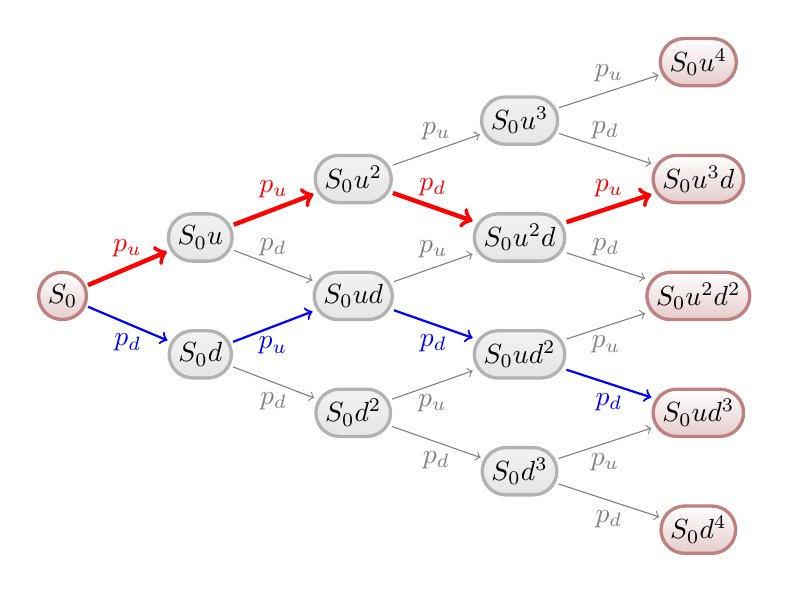
\begin{tikzpicture}
	\matrix[column sep=10mm,row sep=1mm] (tree){
		& & & & \node[term] (u4) {$S_0u^4$}; \\
		& & & \node[nterm] (u3) {$S_0u^3$}; & \\
		& & \node[nterm] (u2) {$S_0u^2$}; & & \node[term] (u3d) {$S_0u^3d$}; \\
		& \node[nterm] (u) {$S_0u$}; & & \node[nterm] (u2d) {$S_0u^2d$};\\
		\node[term] (s) {$S_0$}; & & \node[nterm] (ud) {$S_0ud$}; & & \node[term] (u2d2) {$S_0u^2d^2$}; \\
		& \node[nterm] (d) {$S_0d$}; & &	\node[nterm] (ud2) {$S_0ud^2$};\\
		& & \node[nterm] (d2) {$S_0d^2$}; & & \node[term] (ud3) {$S_0ud^3$}; \\
		& & & \node[nterm] (d3) {$S_0d^3$}; & \\
		& & & & \node[term] (d4) {$S_0d^4$}; \\
	};
	% Lines out of s
	\draw[->,red,ultra thick] (s) -- (u) node[midway,above] {$p_u$};
	\draw[->,blue,thick] (s) -- (d) node[midway,below] {$p_d$};
	% Lines out of u
	\draw[->,red,ultra thick] (u) -- (u2) node[midway,above] {$p_u$};
	\draw[->,gray] (u) -- (ud) node[midway,above] {$p_d$};
	% Lines out of d
	\draw[->,blue,thick] (d) -- (ud) node[midway,below] {$p_u$};
	\draw[->,gray] (d) -- (d2) node[midway,below] {$p_d$};
	% Lines out of u2
	\draw[->,gray] (u2) -- (u3) node[midway,above] {$p_u$};
	\draw[->,red,ultra thick] (u2) -- (u2d) node[midway,above] {$p_d$};
	% Lines out of ud
	\draw[->,gray] (ud) -- (u2d) node[midway,above] {$p_u$};
	\draw[->,blue,thick] (ud) -- (ud2) node[midway,below] {$p_d$};
	% Lines out of d2
	\draw[->,gray] (d2) -- (ud2) node[midway,below] {$p_u$};
	\draw[->,gray] (d2) -- (d3) node[midway,below] {$p_d$};
	% Lines out of u3
	\draw[->,gray] (u3) -- (u4) node[midway,above] {$p_u$};
	\draw[->,gray] (u3) -- (u3d) node[midway,above] {$p_d$};
	% Lines out of u2d
	\draw[->,red,ultra thick] (u2d) -- (u3d) node[midway,above] {$p_u$};
	\draw[->,gray] (u2d) -- (u2d2) node[midway,above] {$p_d$};
	% Lines out of ud2
	\draw[->,gray] (ud2) -- (u2d2) node[midway,below] {$p_u$};
	\draw[->,blue,thick] (ud2) -- (ud3) node[midway,below] {$p_d$};
	% Lines out of d3
	\draw[->,gray] (d3) -- (ud3) node[midway,below] {$p_u$};
	\draw[->,gray] (d3) -- (d4) node[midway,below] {$p_d$};
\end{tikzpicture}


% Recombining 2-step binomial tree for Cox-Ross-Rubinstein model
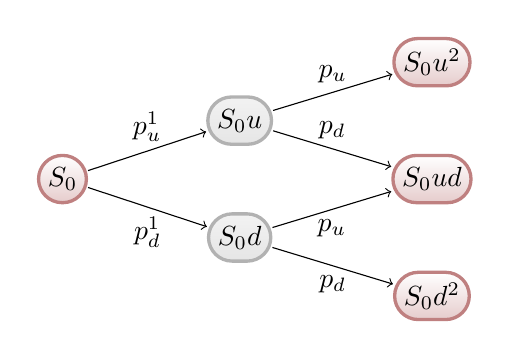
\begin{tikzpicture}
	\matrix[column sep=15mm,row sep=1mm] (tree) {
		& & \node[term] (u2) {$S_0u^2$}; \\
		& \node[nterm] (u) {$S_0u$}; & \\
		\node[term] (s) {$S_0$}; & & \node[term] (ud) {$S_0ud$}; \\
		& \node[nterm] (d) {$S_0d$}; & \\
		& & \node[term] (d2) {$S_0d^2$}; \\
	};
	% Lines out of s
	\draw[->] (s) -- (u) node[midway,above] {$p_u^1$};
	\draw[->] (s) -- (d) node[midway,below] {$p_d^1$};
	% Lines out of u
	\draw[->] (u) -- (u2) node[midway,above] {$p_u$};
	\draw[->] (u) -- (ud) node[midway,above] {$p_d$};
	% Lines out of d
	\draw[->] (d) -- (ud) node[midway,below] {$p_u$};
	\draw[->] (d) -- (d2) node[midway,below] {$p_d$};
\end{tikzpicture}


% Non-recombining 2-step binomial tree for Cox-Ross-Rubinstein model - no criss-cross
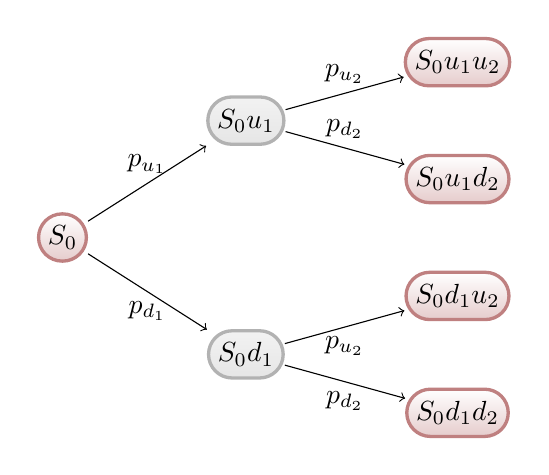
\begin{tikzpicture}
	\matrix[column sep=15mm,row sep=1mm] (tree) {
		& & \node[term] (u2) {$S_0u_1u_2$}; \\
		& \node[nterm] (u) {$S_0u_1$}; & \\
		& & \node[term] (ud) {$S_0u_1d_2$}; \\
		\node[term] (s) {$S_0$}; & & \\
		& & \node[term] (du) {$S_0d_1u_2$}; \\
		& \node[nterm] (d) {$S_0d_1$}; & \\
		& & \node[term] (d2) {$S_0d_1d_2$}; \\
	};
	% Lines out of s
	\draw[->] (s) -- (u) node[midway,above] {$p_{u_1}$};
	\draw[->] (s) -- (d) node[midway,below] {$p_{d_1}$};
	% Lines out of u
	\draw[->] (u) -- (u2) node[midway,above] {$p_{u_2}$};
	\draw[->] (u) -- (ud) node[midway,above] {$p_{d_2}$};
	% Lines out of d
	\draw[->] (d) -- (du) node[midway,below] {$p_{u_2}$};
	\draw[->] (d) -- (d2) node[midway,below] {$p_{d_2}$};
\end{tikzpicture}


% Non-recombining 2-step binomial tree for Cox-Ross-Rubinstein model - criss-cross
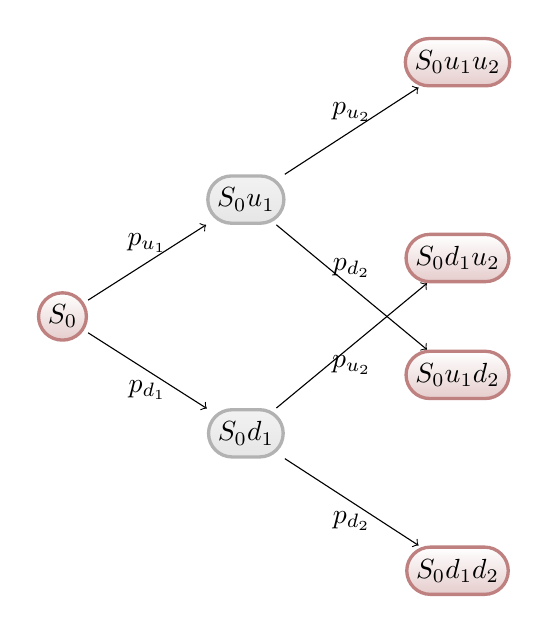
\begin{tikzpicture}
	\matrix[column sep=15mm,row sep=1mm] (tree) {
		& & \node[term] (u2) {$S_0u_1u_2$}; \\
		& & \node {} ; \\
		& & \node {} ; \\
		& & \node {} ; \\
		& \node[nterm] (u) {$S_0u_1$}; & \\
		& & \node[term] (du) {$S_0d_1u_2$}; \\
		\node[term] (s) {$S_0$}; & & \\
		& & \node[term] (ud) {$S_0u_1d_2$}; \\
		& \node[nterm] (d) {$S_0d_1$}; & \\
		& & \node {} ; \\
		& & \node {} ; \\
		& & \node {} ; \\
		& & \node[term] (d2) {$S_0d_1d_2$}; \\
	};
	% Lines out of s
	\draw[->] (s) -- (u) node[midway,above] {$p_{u_1}$};
	\draw[->] (s) -- (d) node[midway,below] {$p_{d_1}$};
	% Lines out of u
	\draw[->] (u) -- (u2) node[midway,above] {$p_{u_2}$};
	\draw[->] (u) -- (ud) node[midway,above] {$p_{d_2}$};
	% Lines out of d
	\draw[->] (d) -- (du) node[midway,below] {$p_{u_2}$};
	\draw[->] (d) -- (d2) node[midway,below] {$p_{d_2}$};
\end{tikzpicture}


% Convex function
\begin{tikzpicture}
	% Draw axes
	\draw [thick, <->] (0,4) -- (0,0) -- (8,0);
	% Plot the function
	\draw (1,15/16) -- (2,1) -- (5,2) -- (7,3) -- (8,4);
  \draw[red,dashed] (2,1) -- (7,3);
  \draw (1,15/16) -- (2,1) -- (5,2) -- (7,3) -- (8,4);
\end{tikzpicture}


\end{document}

%%% Local Variables:
%%% mode: latex
%%% TeX-master: t
%%% End:
